\documentclass{ximera}

\title{Practice for Advanced Linear Algebra}

%\auor{Matthew Charnley and Jason Nowell}
\usepackage[margin=1.5cm]{geometry}
\usepackage{indentfirst}
\usepackage{sagetex}
\usepackage{lipsum}
\usepackage{amsmath}
\usepackage{mathrsfs}


%%% Random packages added without verifying what they are really doing - just to get initial compile to work.
\usepackage{tcolorbox}
\usepackage{hypcap}
\usepackage{booktabs}%% To get \toprule,\midrule,\bottomrule etc.
\usepackage{nicefrac}
\usepackage{caption}
\usepackage{units}

% This is my modified wrapfig that doesn't use intextsep
\usepackage{mywrapfig}
\usepackage{import}



%%% End to random added packages.


\graphicspath{
    {./figures/}
    {./../figures/}
    {./../../figures/}
}
\renewcommand{\log}{\ln}%%%%
\DeclareMathOperator{\arcsec}{arcsec}
%% New commands


%%%%%%%%%%%%%%%%%%%%
% New Conditionals %
%%%%%%%%%%%%%%%%%%%%


% referencing
\makeatletter
    \DeclareRobustCommand{\myvref}[2]{%
      \leavevmode%
      \begingroup
        \let\T@pageref\@pagerefstar
        \hyperref[{#2}]{%
	  #1~\ref*{#2}%
        }%
        \vpageref[\unskip]{#2}%
      \endgroup
    }%

    \DeclareRobustCommand{\myref}[2]{%
      \leavevmode%
      \begingroup
        \let\T@pageref\@pagerefstar
        \hyperref[{#2}]{%
	  #1~\ref*{#2}%
        }%
      \endgroup
    }%
\makeatother

\newcommand{\figurevref}[1]{\myvref{Figure}{#1}}
\newcommand{\figureref}[1]{\myref{Figure}{#1}}
\newcommand{\tablevref}[1]{\myvref{Table}{#1}}
\newcommand{\tableref}[1]{\myref{Table}{#1}}
\newcommand{\chapterref}[1]{\myref{chapter}{#1}}
\newcommand{\Chapterref}[1]{\myref{Chapter}{#1}}
\newcommand{\appendixref}[1]{\myref{appendix}{#1}}
\newcommand{\Appendixref}[1]{\myref{Appendix}{#1}}
\newcommand{\sectionref}[1]{\myref{\S}{#1}}
\newcommand{\subsectionref}[1]{\myref{subsection}{#1}}
\newcommand{\subsectionvref}[1]{\myvref{subsection}{#1}}
\newcommand{\exercisevref}[1]{\myvref{Exercise}{#1}}
\newcommand{\exerciseref}[1]{\myref{Exercise}{#1}}
\newcommand{\examplevref}[1]{\myvref{Example}{#1}}
\newcommand{\exampleref}[1]{\myref{Example}{#1}}
\newcommand{\thmvref}[1]{\myvref{Theorem}{#1}}
\newcommand{\thmref}[1]{\myref{Theorem}{#1}}


\renewcommand{\exampleref}[1]{ {\color{red} \bfseries Normally a reference to a previous example goes here.}}
\renewcommand{\figurevref}[1]{ {\color{red} \bfseries Normally a reference to a previous figure goes here.}}
\renewcommand{\tablevref}[1]{ {\color{red} \bfseries Normally a reference to a previous table goes here.}}
\renewcommand{\Appendixref}[1]{ {\color{red} \bfseries Normally a reference to an Appendix goes here.}}
\renewcommand{\exercisevref}[1]{ {\color{red} \bfseries Normally a reference to a previous exercise goes here.}}



\newcommand{\R}{\mathbb{R}}

%% Example Solution Env.
\def\beginSolclaim{\par\addvspace{\medskipamount}\noindent\hbox{\bf Solution:}\hspace{0.5em}\ignorespaces}
\def\endSolclaim{\par\addvspace{-1em}\hfill\rule{1em}{0.4pt}\hspace{-0.4pt}\rule{0.4pt}{1em}\par\addvspace{\medskipamount}}
\newenvironment{exampleSol}[1][]{\beginSolclaim}{\endSolclaim}

%% General figure formating from original book.
\newcommand{\mybeginframe}{%
\begin{tcolorbox}[colback=white,colframe=lightgray,left=5pt,right=5pt]%
}
\newcommand{\myendframe}{%
\end{tcolorbox}%
}

%%% Eventually return and fix this to make matlab code work correctly.
%% Define the matlab environment as another code environment
%\newenvironment{matlab}
%{% Begin Environment Code
%{ \centering \bfseries Matlab Code }
%\begin{code}
%}% End of Begin Environment Code
%{% Start of End Environment Code
%\end{code}
%}% End of End Environment Code


% this one should have a caption, first argument is the size
\newenvironment{mywrapfig}[2][]{
 \wrapfigure[#1]{r}{#2}
 \mybeginframe
 \centering
}{%
 \myendframe
 \endwrapfigure
}

% this one has no caption, first argument is size,
% the second argument is a larger size used for HTML (ignored by latex)
\newenvironment{mywrapfigsimp}[3][]{%
 \wrapfigure[#1]{r}{#2}%
 \centering%
}{%
 \endwrapfigure%
}
\newenvironment{myfig}
    {%
    \begin{figure}[h!t]
        \mybeginframe%
        \centering%
    }
    {%
        \myendframe
    \end{figure}%
    }


% graphics include
\newcommand{\diffyincludegraphics}[3]{\includegraphics[#1]{#3}}
\newcommand{\myincludegraphics}[3]{\includegraphics[#1]{#3}}
\newcommand{\inputpdft}[1]{\subimport*{../figures/}{#1.pdf_t}}


%% Not sure what these even do? They don't seem to actually work... fun!
%\newcommand{\mybxbg}[1]{\tcboxmath[colback=white,colframe=black,boxrule=0.5pt,top=1.5pt,bottom=1.5pt]{#1}}
%\newcommand{\mybxsm}[1]{\tcboxmath[colback=white,colframe=black,boxrule=0.5pt,left=0pt,right=0pt,top=0pt,bottom=0pt]{#1}}
\newcommand{\mybxsm}[1]{#1}
\newcommand{\mybxbg}[1]{#1}

%%% Something about tasks for practice/hw?
\usepackage{tasks}
\usepackage{footnote}
\makesavenoteenv{tasks}


%% For pdf only?
\newcommand{\diffypdfversion}[1]{#1}


%% Kill ``cite'' and go back later to fix it.
\renewcommand{\cite}[1]{}


%% Currently we can't really use index or its derivatives. So we are gonna kill them off.
\renewcommand{\index}[1]{}
\newcommand{\myindex}[1]{#1}







\begin{document}
\begin{abstract}
Why?
\end{abstract}
\maketitle

\begin{exercise}
    Take the equation $m x'' + c x' + kx = 0$, with $m > 0$, $c \geq 0$, $k > 0$ for the mass-spring system.
    \begin{itemize}
        \item Convert this to a system of first order equations.\\
        ${\vec{x}}' = \left[\begin{smallmatrix} \answer{0} & \answer{1} \\ \answer{-\frac{k}{m}} & \answer{-\frac{c}{m}} \end{smallmatrix}\right]\vec{x}$
        \item Classify for what $m, c, k$ do you get which behavior.\\
        $c=\answer{0}$ is center, $\answer{c^2 - 4mk} < \answer{0}$ is spiral sink, $\answer{c^2 - 4mk} = \answer{0}$ is improper sink, $\answer{c^2 - 4mk} > \answer{0}$ is nodal sink.
        \item Can you explain from physical intuition why you do not get all the different kinds of behavior here?
    \end{itemize}
\end{exercise}
%\comboSol
%{%
%a)~${\vec{x}}' = \left[\begin{smallmatrix} 0 & 1 \\ -k/m &-c/m \end{smallmatrix}\right]\vec{x}$ \quad b)~$c=0$ is center, $c^2 - 4mk < 0$ is spiral sink, $c^2 - 4mk = 0$ is improper sink, $c^2 - 4mk > 0$ is nodal sink. \quad c)~The forced positive coefficients restricts the behavior 
%}

\begin{exercise}
    What happens in the case when $P = \left[ \begin{smallmatrix} 1 & 1 \\ 0 & 1 \end{smallmatrix} \right]$?  In this case the eigenvalue is repeated and there is only one independent eigenvector. What picture does this look like?
\end{exercise}
%\comboSol
%{%
%Improper nodal sink \hfill\raisebox{-0.5\height}{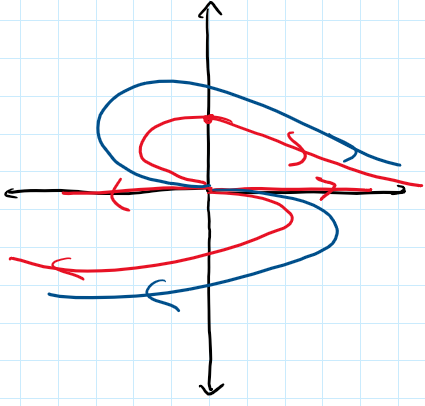
\includegraphics[height=1.5in]{Images/phaseportrait_1_1_0_1_sketch.png}}\hfill\hfill
%}

\begin{exercise}
    What happens in the case when $P = \left[ \begin{smallmatrix} 1 & 1 \\ 1 & 1 \end{smallmatrix} \right]$? Does this look like any of the pictures we have drawn?
\end{exercise}
%\comboSol
%{%
%It does not look like any of our previous pictures. \hfill\raisebox{-0.5\height}{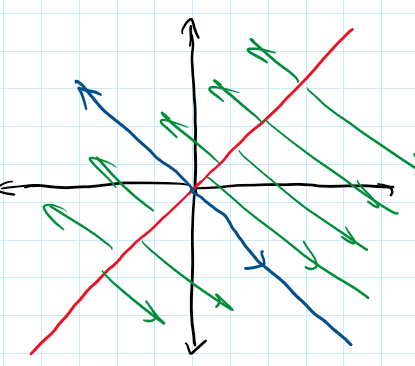
\includegraphics[height=1.5in]{Images/phaseportrait_1_1_1_1_sketch.png}}\hfill\hfill
%}

\begin{exercise}%
    Describe the behavior of the following systems without solving:
    \begin{itemize}
        \item $x' = x + y$, \quad $y' = x-y$.\\
        The eigenvalues are: $\pm \answer{\sqrt{3}}$, so the behavior is a \wordChoice{\choice{center/ellipses}\choice{source}\choice{sink}[correct]\choice{saddle}}.
        \item $x_1' = x_1 + x_2$, \quad $x_2' = 2 x_2$.\\
        The eigenvalues are: $\answer{1}$, $\answer{2}$, so the behavior is a \wordChoice{\choice{center/ellipses}\choice[correct]{source}\choice{sink}\choice{saddle}}.
        \item $x_1' = -2x_2$, \quad $x_2' = 2 x_1$.\\
        The eigenvalues are: $\pm \answer{2i}$, so the behavior is a \wordChoice{\choice[correct]{center/ellipses}\choice{source}\choice{sink}\choice{saddle}}.
        \item $x' = x + 3y$, \quad $y' = -2x-4y$.\\
        The eigenvalues are: $\pm \answer{-2}$, $\answer{-1}$, so the behavior is a \wordChoice{\choice{center/ellipses}\choice{source}\choice[correct]{sink}\choice{saddle}}.
        \item $x' = x - 4y$, \quad $y' = -4x+y$.\\
        The eigenvalues are: $\pm \answer{-3}$, $\answer{5}$, so the behavior is a \wordChoice{\choice{center/ellipses}\choice{source}\choice{sink}\choice[correct]{saddle}}.
    \end{itemize}
\end{exercise}
%\exsol{%
%a) Two eigenvalues: $\pm \sqrt{2}$ so the behavior is a saddle.
%\quad
%b) Two eigenvalues: $1$ and $2$, so the behavior is a source.
%\quad
%c) Two eigenvalues: $\pm 2i$, so the behavior is a center (ellipses).
%\quad
%d) Two eigenvalues: $-1$ and $-2$, so the behavior is a sink.
%\quad
%e) Two eigenvalues: $5$ and $-3$, so the behavior is a saddle.
%}

\begin{exercise}
    Which behaviors are possible if $P$ is diagonal, that is $P = \left[ \begin{smallmatrix} a & 0 \\ 0 & b \end{smallmatrix} \right]$? You can assume that $a$ and $b$ are not zero.\\
    The eigenvalues are: $\pm \answer{a}$, $\answer{b}$, so the behavior is a \wordChoice{\choice{center/ellipses}\choice{source}\choice{sink}\choice{saddle}\choice[correct]{Any behavior is possible.}}.
\end{exercise}
%\comboSol
%{%
%Eigenvalues are $a$ and $b$, so any real eigenvalue behavior is possible. Saddle, source, sink.
%}

\begin{exercise}%
    Suppose that $\vec{x}\,' = A \vec{x}$ where $A$ is a 2 by 2 matrix with eigenvalues $2\pm i$.  Describe the behavior.\\
    The behavior is a \wordChoice{\choice{center/ellipses}\choice[correct]{source}\choice{sink}\choice{saddle}\choice{Any behavior is possible.}}.
\end{exercise}
%\exsol{%
%Spiral source.
%}

\begin{exercise}\label{ex:TwoDimSys1}%
    For each of the following matrices $A$, describe the behavior and classify the phase portrait of the system given by ${\vec{x}}' = A\vec{x}$. Use the eigenvalues to determine this.
    \begin{itemize}
        \item $A = \begin{bmatrix} 7 & -8 \\ 3 & -3 \end{bmatrix}$\\
        The behavior is a \wordChoice{\choice[correct]{Nodal},\choice{Improper Nodal},\choice{Spiral},\choice{None of these choices}} \wordChoice{\choice{center/ellipses}\choice[correct]{source}\choice{sink}\choice{saddle}\choice{Any behavior is possible}}.
        \item $A = \begin{bmatrix} 3 & 5 \\ -1 & 1 \end{bmatrix}$\\
        The behavior is a \wordChoice{\choice{Nodal},\choice{Improper Nodal},\choice[correct]{Spiral},\choice{None of these choices}} \wordChoice{\choice{center/ellipses}\choice[correct]{source}\choice{sink}\choice{saddle}\choice{Any behavior is possible}}.
        \item $A = \begin{bmatrix} 8 & -18 \\ 4 & -10 \end{bmatrix}$\\
        The behavior is a \wordChoice{\choice{Nodal},\choice{Improper Nodal},\choice{Spiral},\choice{None of these choices}} \wordChoice{\choice{center/ellipses}\choice{source}\choice{sink}\choice[correct]{saddle}\choice{Any behavior is possible.}}.
        \item $A = \begin{bmatrix} -2 & -4 \\0 & -3 \end{bmatrix}$\\
        The behavior is a \wordChoice{\choice[correct]{Nodal},\choice{Improper Nodal},\choice{Spiral},\choice{None of these choices}} \wordChoice{\choice{center/ellipses}\choice{source}\choice[correct]{sink}\choice{saddle}\choice{Any behavior is possible}}.
        \item $A = \begin{bmatrix} 3 & -2 \\ 2 & -3 \end{bmatrix}$\\
        The behavior is a \wordChoice{\choice{Nodal},\choice{Improper Nodal},\choice[correct]{Spiral},\choice{None of these choices}} \wordChoice{\choice{center/ellipses}\choice{source}\choice[correct]{sink}\choice{saddle}\choice{Any behavior is possible}}.
        \item $A = \begin{bmatrix} -3 & -4 \\ 1 & 1 \end{bmatrix}$\\
        The behavior is a \wordChoice{\choice{Nodal},\choice[correct]{Improper Nodal},\choice{Spiral},\choice{None of these choices}} \wordChoice{\choice{center/ellipses}\choice{source}\choice[correct]{sink}\choice{saddle}\choice{Any behavior is possible}}.
    \end{itemize}
\end{exercise}
%\exsol{%
%a) Nodal source \quad c) Spiral source  \quad  c) Saddle \quad d) Nodal sink \quad  e) Spiral sink \quad f) Improper nodal sink
%}

\begin{exercise}
For each of the matrices and systems in exercise \ref{ex:TwoDimSys1}, perform the same analysis using the trace and determinant of the matrix.
\end{exercise}

\begin{exercise}
    Consider the system of differential equations given by 
    \begin{equation*}
        {\vec{x}}'  = \begin{bmatrix} -2 & -3 \\ 3 & -2 \end{bmatrix} \vec{x}.
    \end{equation*}
    \begin{itemize}
        \item Use trace and determinant analysis to determine the behavior of this linear system. \\
        The behavior is a \wordChoice{\choice{Nodal},\choice{Improper Nodal},\choice[correct]{Spiral},\choice{None of these choices}} \wordChoice{\choice{center/ellipses}\choice{source}\choice[correct]{sink}\choice{saddle}\choice{Any behavior is possible}}.
        \item Find the general solution to this system of differential equations and verify that it matches the analysis in (a). [ Use $A$ and $B$ for arbitrary constants]\\
        $\vec{x}(t) = \answer{Ae^{-2t}}\left[\begin{smallmatrix} \answer{-\sin(3t)} \\ \cos(3t) \end{smallmatrix}\right] + \answer{Be^{-2t}} \left[\begin{smallmatrix} \answer{\cos(3t)} \\ \sin(3t) \end{smallmatrix}\right]$.
    \end{itemize}
\end{exercise}
%\comboSol
%{%
%Spiral sink. $\vec{x}(t) = C_1e^{-2t}\left[\begin{smallmatrix} -\sin(3t) \\ \cos(3t) \end{smallmatrix}\right] + C_2e^{-2t} \left[\begin{smallmatrix} \cos(3t) \\ \sin(3t) \end{smallmatrix}\right]$.
%}

\begin{exercise}
    Consider the system of differential equations given by 
    \begin{equation*}
        {\vec{x}}'  = \begin{bmatrix} -2 & -3 \\ 3 & 4 \end{bmatrix} \vec{x}.
    \end{equation*}
    \begin{itemize}
        \item Use trace and determinant analysis to determine the behavior of this linear system.\\
        The behavior is a \wordChoice{\choice[correct]{Nodal},\choice{Improper Nodal},\choice{Spiral},\choice{None of these choices}} \wordChoice{\choice{center/ellipses}\choice[correct]{source}\choice{sink}\choice{saddle}\choice{Any behavior is possible.}}.
        \item Find the general solution to this system of differential equations and verify that it matches the analysis in (a). [ Use $A$ and $B$ for arbitrary constants]\\
        $\vec{x}(t) = \answer{A} \left[\begin{smallmatrix} \answer{1} \\ -1 \end{smallmatrix}\right]e^t + \answer{B}\left(\left[\begin{smallmatrix} 1 \\ \answer{-1} \end{smallmatrix}\right]te^t + \left[\begin{smallmatrix} \answer{-\frac{1}{3}} \\ 0 \end{smallmatrix}\right]e^t \right)$
    \end{itemize}
\end{exercise}
%\comboSol
%{%
%Improper nodal source. $\vec{x}(t) = C_1 \left[\begin{smallmatrix} 1 \\ -1 \end{smallmatrix}\right]e^t + C_2\left(\left[\begin{smallmatrix} 1 \\ -1 \end{smallmatrix}\right]te^t + \left[\begin{smallmatrix} -1/3 \\ 0 \end{smallmatrix}\right]e^t \right)$
%}

\begin{exercise}
    Take the system from example \ref{sintro:closedbrine-example}, $x_1'=\frac{r}{V}(x_2-x_1)$, $x_2'=\frac{r}{V}(x_1-x_2)$. As we said, one of the eigenvalues is zero.  What is the other eigenvalue, how does the picture look like and what happens when $t$ goes to infinity.
\end{exercise}
%\comboSol
%{%
%All solutions flow directly to the line $y=x$.
%}

\begin{exercise}%
    Take 
    $\left[ 
    \begin{smallmatrix}
        x \\ 
        y 
    \end{smallmatrix}
    \right] '
    = \left[ 
    \begin{smallmatrix} 
        0 & 1 \\ 
        0 & 0
    \end{smallmatrix}
    \right] \left[ 
    \begin{smallmatrix}
        x \\ 
        y 
    \end{smallmatrix}\right]$.
    Draw the vector field and describe the behavior.  Is it one of the behaviors that we have seen before?
\end{exercise}
%\exsol{%
%\\[6pt]
%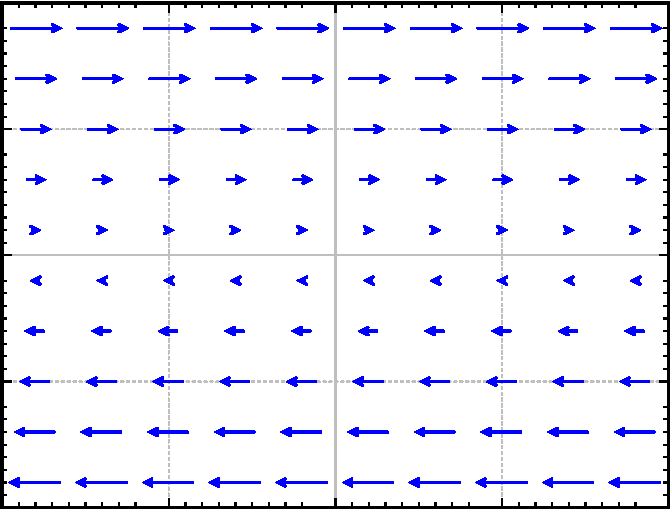
\includegraphics[width=2in]{figures/0100vectorfield}
%\\
%The solution does not move anywhere if $y = 0$.  When $y$ is positive,
%the solution moves (with constant speed)
%in the positive $x$ direction.  When $y$ is
%negative, the solution moves (with constant speed) in the negative
%$x$ direction.  It is not one of the behaviors we have seen.
%\\
%Note that the matrix has a double eigenvalue 0 and the general solution is
%$x = C_1 t + C_2$ and $y = C_1$, which agrees with the
%description above.
%}

\begin{exercise}
    In this exercise, we will analyze ``perturbations'' or near-by matrices to the ones that are given. This will be important later in section \ref{linearization:section}. For each of the following matrices
    \begin{itemize}
        \item Find the trace and determinant, and use them to classify the behavior of the linear system ${\vec{x}}' = A\vec{x}$ for the given matrix $A$.
        \item Draw a sketch of the trace-determinant plane, including the curve $D = \frac{T^2}{4}$, and plot the point corresponding to the matrix on those axes.
        \item Look at the points in a small (as small as you want) circle around the point you just drew. What does the behavior look like for systems whose matrices fall within that circle? What do these behaviors have in common with each other, and how do they differ?
    \end{itemize}
    \begin{equation*}
    \begin{split}
        (i)\ \begin{bmatrix} 2 & 8 \\ -3 & -8 \end{bmatrix} \qquad (ii)\ \begin{bmatrix} 15 & -12 \\ 16 & -13 \end{bmatrix} \qquad &(iii)\ \begin{bmatrix} 2 & -1 \\ 5 & -2 \end{bmatrix} \qquad (iv)\ \begin{bmatrix} 4 & -1 \\ 2 & 2 \end{bmatrix}\\
        (v)\ \begin{bmatrix} -2 & 2 \\ -2 & -6 \end{bmatrix} \qquad (vi)\ \begin{bmatrix} -1 & -4 \\ 2 & 5 \end{bmatrix} \qquad &(vii)\ \begin{bmatrix} -5 & 6 \\ -3 & 1 \end{bmatrix} \qquad (viii)\ \begin{bmatrix} 5 & -2 \\ 8 & -3 \end{bmatrix} 
    \end{split}
    \end{equation*}
    \begin{itemize}
        \item[i]  $T=\answer{-6}$, $D = \answer{8}$. 
            The behavior is a \wordChoice{\choice[correct]{Nodal},\choice{Improper Nodal},\choice{Spiral},\choice{None of these choices}} \wordChoice{\choice{center/ellipses}\choice{source}\choice[correct]{sink}\choice{saddle}\choice{Any behavior is possible}}.
            \begin{feedback}[correct]
                All points nearby are nodal sinks. 
            \end{feedback}
        \item[ii]  $T=\answer{2}$, $D = \answer{-3}$. 
            The behavior is a \wordChoice{\choice{Nodal},\choice{Improper Nodal},\choice{Spiral},\choice[correct]{None of these choices}} \wordChoice{\choice{center/ellipses}\choice{source}\choice{sink}\choice[correct]{saddle}\choice{Any behavior is possible}}.
            \begin{feedback}[correct]
                All points nearby are saddles. 
            \end{feedback}
        \item[iii]  $T=\answer{-6}$, $D = \answer{8}$. 
            The behavior is a \wordChoice{\choice{Nodal},\choice{Improper Nodal},\choice{Spiral},\choice[correct]{None of these choices}} \wordChoice{\choice[correct]{center/ellipses}\choice{source}\choice{sink}\choice{saddle}\choice{Any behavior is possible}}.
            \begin{feedback}[correct]
                Points nearby are all spirals, but they could be asymptotically stable, centers, or unstable. Stability is unknown.
            \end{feedback}
        \item[iv]  $T=\answer{-6}$, $D = \answer{8}$. 
            The behavior is a \wordChoice{\choice{Nodal},\choice{Improper Nodal},\choice[correct]{Spiral},\choice{None of these choices}} \wordChoice{\choice{center/ellipses}\choice[correct]{source}\choice{sink}\choice{saddle}\choice{Any behavior is possible}}.
            \begin{feedback}[correct]
                Spiral source. All points nearby are spiral sources.
            \end{feedback}
         \item[v]  $T=\answer{-6}$, $D = \answer{8}$. 
             The behavior is a \wordChoice{\choice{Nodal},\choice[correct]{Improper Nodal},\choice{Spiral},\choice{None of these choices}} \wordChoice{\choice{center/ellipses}\choice{source}\choice[correct]{sink}\choice{saddle}\choice{Any behavior is possible}}.
            \begin{feedback}[correct]
                All points nearby will be asymptotically stable, but they could be nodal sinks, improper nodal sinks, or spiral sinks.
            \end{feedback}
        \item[vi]  $T=\answer{-6}$, $D = \answer{8}$. 
            The behavior is a \wordChoice{\choice[correct]{Nodal},\choice{Improper Nodal},\choice{Spiral},\choice{None of these choices}} \wordChoice{\choice{center/ellipses}\choice[correct]{source}\choice{sink}\choice{saddle}\choice{Any behavior is possible}}.
            \begin{feedback}[correct]
                All points nearby are nodal sources.
            \end{feedback}
         \item[vii]  $T=\answer{-6}$, $D = \answer{8}$. 
             The behavior is a \wordChoice{\choice{Nodal},\choice{Improper Nodal},\choice[correct]{Spiral},\choice{None of these choices}} \wordChoice{\choice{center/ellipses}\choice{source}\choice[correct]{sink}\choice{saddle}\choice{Any behavior is possible}}.
            \begin{feedback}[correct]
                Spiral sink. All points nearby are spiral sinks.
            \end{feedback}
        \item[viii]  $T=\answer{-6}$, $D = \answer{8}$. 
            The behavior is a \wordChoice{\choice{Nodal},\choice[correct]{Improper Nodal},\choice{Spiral},\choice{None of these choices}} \wordChoice{\choice{center/ellipses}\choice[correct]{source}\choice{sink}\choice{saddle}\choice{Any behavior is possible}}.
            \begin{feedback}[correct]
                All points nearby will be unstable, but they may be spirals, nodal sources, or improper nodal sources.
            \end{feedback}
    \end{itemize}
\end{exercise}
%\exsol{%
%(i) $T=-6$, $D = 8$. Nodal sink. All points nearby are nodal sinks. \\
%(ii)  $T = 2$, $D = -3$. Saddle. All points nearby are saddles. \\
%(iii)  $T = 0$, $D = 1$. Center. Points nearby are all spirals, but they could be asymptotically stable, centers, or unstable. Stability is unknown.\\
%(iv)  $T = 6$, $D = 10$. Spiral source. All points nearby are spiral sources.\\
%(v)  $T = -8$, $D = 16$. Improper nodal sink. All points nearby will be asymptotically stable, but they could be nodal sinks, improper nodal sinks, or spiral sinks.\\
%(vi)  $T = 4$, $D = 3$. Nodal source. All points nearby are nodal sources. \\
%(vii)  $T = -4$, $D = 13$. Spiral sink. All points nearby are spiral sinks. \\
%(viii)  $T = 2$, $D = 1$. Improper nodal source. All points nearby will be unstable, but they may be spirals, nodal sources, or improper nodal sources.\\
%}%



\end{document}